\documentclass[t,11pt,eleve]{article}
\RequirePackage{geometry}
\geometry{a4paper,top=2cm,bottom=2cm,left=2cm,right=2cm}
\RequirePackage{amsmath,amssymb}
\RequirePackage{amsfonts}
\RequirePackage{graphicx}
\usepackage[T1]{fontenc} 
\usepackage[utf8]{inputenc}
\usepackage[frenchb]{babel}
\usepackage{pifont}
\usepackage{colortbl}  
\usepackage{lmodern} %%% ajoute cette ligne dans ton préambule

\usepackage{multicol}
\usepackage{ulem}
\usepackage{url}
\usepackage{amsmath} 
\usepackage{stmaryrd}
\normalem

\parindent=0pt

\RequirePackage{framed}


\newcommand{\FIG}[1]{\textsc{Figure} {\upshape\ref{#1}}}
\usepackage{numprint} %affichage de nombres correctement avec \numprint{}

%\usepackage{picins}    %permet d'insérer une image à coté d'un texte \parpic[r]{\includegraphics{}}texte...
\usepackage{tikz}
\usetikzlibrary{calc}
% Unités
\usepackage[locale = FR]{siunitx}
\sisetup{inter-unit-product = \ensuremath{{}\cdot{}}}
\usepackage{numprint} %affichage de nombres correctment avec \numprint{}
\usepackage{multirow}
\definecolor{gris_c}{gray}{0.9}
\definecolor{gris_f}{gray}{0.25}
\definecolor{gris_tc}{gray}{0.96}
\definecolor{gris_ttc}{gray}{0.98}

\newenvironment{activite}[1][\hsize]%
{%
    \def\FrameCommand%
    {%
\rotatebox{90}{\textit{\textsf{REMARQUE}}} 
        {\color{blue}\vrule width 3pt}%
        \hspace{0pt}%must no space.
        \fboxsep=\FrameSep\colorbox{gris_c}%
    }%
    \MakeFramed{\hsize#1\advance\hsize-\width\FrameRestore}%
}%
{\endMakeFramed}%

\newenvironment{donnees}[1][\hsize]%
{%
    \def\FrameCommand%
    {%
\rotatebox{90}{\textit{\textsf{DONNEES}}} 
        {\color{blue}\vrule width 3pt}%
        \hspace{0pt}%must no space.
        \fboxsep=\FrameSep\colorbox{gris_c}%
    }%
    \MakeFramed{\hsize#1\advance\hsize-\width\FrameRestore}%
}%
{\endMakeFramed}%

\newenvironment{objectif}[1][\hsize]%
{%
    \def\FrameCommand%
    {%
\rotatebox{90}{\textit{\textsf{OBJECTIF}}} 
        {\color{blue}\vrule width 3pt}%
        \hspace{0pt}%must no space.
        \fboxsep=\FrameSep\colorbox{gris_c}%
    }%
    \MakeFramed{\hsize#1\advance\hsize-\width\FrameRestore}%
}%
{\endMakeFramed}%


\NeedsTeXFormat{LaTeX2e}


%%% Exemple
\newenvironment{exemple}[1][\hsize]%
{%
    \def\FrameCommand%
    {%
\rotatebox{90}{\textit{\textsf{Exemple}}} 
        {\color{blue}\vrule width 3pt}%
        \hspace{0pt}%must no space.
        \fboxsep=\FrameSep\colorbox{gris_c}%
    }%
    \MakeFramed{\hsize#1\advance\hsize-\width\FrameRestore}%
}%
{\endMakeFramed}%


%% Questions et exercices
\newcounter{numques}%Création d'un compteur qui s'appelle numques
\setcounter{numques}{0}%initialisation du compteur
\newcommand{\question}[1]{%Création d'une macro ayant un paramètre
\addtocounter{numques}{1}%chaque fois que cette macro est appelée, elle ajoute 1 au compteur numexos
\textbf{Question\, \textcolor{black}{\thenumques}\,}\,\textit{#1}\\{\vspace{0cm}}}


\newcounter{numexo}%Création d'un compteur qui s'appelle numques
\setcounter{numexo}{0}%initialisation du compteur
\newcommand{\exer}[1]{%Création d'une macro ayant un paramètre
\refstepcounter{numexo} % incrément compteur et label
%\addtocounter{numexo}{1}%chaque fois que cette macro est appelée, elle ajoute 1 au compteur numexo
\noindent\textsf{\textbf{Exercice\, \textcolor{black}{\thenumexo}\, -- \, #1}}}


\RequirePackage{geometry}
\usepackage{beamerarticle}
%\usepackage{boxedminipage,multicol,pifont}
\renewcommand{\d}{\textrm{d}}
\renewcommand{\baselinestretch}{1.3}
\newcommand{\longueur}{6cm}
\RequirePackage{amsmath,amssymb}
\RequirePackage{amsfonts}
\RequirePackage{graphicx}
%\RequirePackage{mesmacros}
\usepackage[T1]{fontenc} 
\usepackage[utf8]{inputenc}
\usepackage[frenchb]{babel}
\usepackage{pifont}

\RequirePackage{comment}
\RequirePackage{multicol}

\RequirePackage{colortbl}
\RequirePackage{fancybox}
\usepackage{colortbl}


\RequirePackage{tikz,tkz-tab,tkz-fct,tkz-base,tkz-euclide}
%\RequirePackage{tikz,tkz-base,tkz-euclide}

%\RequirePackage{graphe}
\RequirePackage{framed}

\usepackage{ulem}
\normalem


%%%ENTETES%%%
%%%%%%%%%%%
\newcommand{\entetedebut}{
{\noindent \textbf{PTSI2 -- 2019/2020 -- Maths} \hfill Lycée La Martinière-Monplaisir -- Lyon \vspace{2mm}}
\hrule
\begin{center} 
}
\newcommand{\entetedebutinfo}{
{\noindent \textbf{PTSI -- 2023/2024 -- Info} \hfill Lycée La Martinière-Monplaisir -- Lyon \vspace{2mm} }
\hrule
\begin{center} 
}

\newcommand{\entetefin}{
\end{center}
\hrule
\vspace*{0.5cm}
}

\newcommand{\entetedebutsnow}{
\begin{tikzpicture}[decoration=Koch snowflake]
\draw (0,0)--(12,0)node[midway,above]
}

\newcommand{\entetefinsnow}{
\draw decorate{ decorate{ decorate{ decorate{ (12,0)--(17,0) }}}};
\end{tikzpicture}
\vspace*{1cm}
}
%%% Lorqu'on utilise les entetes koch snowflake, il faut juste mettre tout le titre entre { } et un point-virgule à la fin, car on est dans un tikzpicture.
\newcommand{\entetecours}{
\entetedebut
\textbf{\textsf{\Large Ch \numero. \titre.}}
\entetefin
}
\newcommand{\entetecoursinfo}{
\entetedebutinfo
\textbf{\textsf{\Large Ch \numero. \titre.}}
\entetefin
}


\newcommand{\entete}{
\entetedebut
\textbf{\textsf{\Large \titre.}}
\entetefin
}
\newcommand{\enteteinfo}{
\entetedebutinfo
\textbf{\textsf{\Large \titre.}}
\entetefin
}


\newcommand{\entetetd}{
\entetedebut
\textbf{\textsf{\Large TD \numero. \titre.}}
\entetefin
}

\newcommand{\entetetp}{
\entetedebut
\textbf{\textsf{\Large TP \numero. \titre.}}
\entetefin
}

\newcommand{\entetetpinfo}{
\entetedebutinfo
\textbf{\textsf{\Large TP \numero. \titre.}}
\entetefin
}



\newcommand{\enteteindic}{
\entetedebut
\textbf{\textsf{\Large Indications et solutions pour le TD \numero.}}
\entetefin
}


\newcommand{\entetecor}{
\entetedebut
\textbf{\textsf{\Large Corrigés pour le TD \numero.}}
\entetefin
}

%%% Python
\usepackage{listingsutf8}
\lstset{language=Python,
  inputencoding=utf8/latin1,
  breaklines=true,
  basicstyle=\ttfamily\small,
  keywordstyle=\bfseries\color{green!40!black},
  commentstyle=\itshape\color{purple!40!black},
  identifierstyle=\color{blue},
  stringstyle=\color{orange},
  upquote = true,
  columns=fullflexible,
  backgroundcolor=\color{gray!10},frame=leftline,rulecolor=\color{gray}}  
  

\lstset{
     literate=%
         {é}{{\'e}}1    
         {è}{{\`e}}1    
         {ê}{{\^e}}1    
         {à}{{\`a}}1    
         {ô}{{\^o}}1    
         {ù}{{\`u}}1    
}
%%%%%%%%%%%%%%%%%%%%%%%%%%%%%%%%%%%%%%%
\parindent=0pt

\newlength{\myline}


\newcommand{\graphetext}[3]{
\setlength{\myline}{\linewidth}
\addtolength{\myline}{-1cm}
\addtolength{\myline}{-#1}
\begin{tabular}{ll}
\parbox[c]{#1}{\includegraphics[width=#1]{#2}}&
\parbox[c]{\myline}{#3}
\end{tabular}}
\newcommand{\tikztexte}[3]{
\setlength{\myline}{\linewidth}
\addtolength{\myline}{-1cm}
\addtolength{\myline}{-#1}
\begin{tabular}{ll}
\parbox[c]{#1}{#2}&
\parbox[c]{\myline}{#3}
\end{tabular}}
\newcommand{\textgraphe}[3]{
\setlength{\myline}{\linewidth}
\addtolength{\myline}{-.5cm}
\addtolength{\myline}{-#1}
\begin{tabular}{ll}
\parbox[c]{\myline}{#2}&
\parbox[c]{#1}{\includegraphics[width=#1]{#3}}
\end{tabular}}
\newcommand{\textetikz}[3]{
\setlength{\myline}{\linewidth}
\addtolength{\myline}{-.5cm}
\addtolength{\myline}{-#1}
\begin{tabular}{ll}
\parbox[c]{\myline}{#2}&
\parbox[c]{#1}{#3}
\end{tabular}}
\newcommand{\p}{\pause}


%%%NUMEROTATION DES PARTIES%%%
\renewcommand{\thesection}{\hspace{-0.6cm}\arabic{section}}
\renewcommand{\thesubsection}{\hspace{-0.4cm}\arabic{section}.\alph{subsection}}
\renewcommand{\thesubsubsection}{\hspace{0cm}\arabic{section}.\alph{subsection}.\roman{subsubsection}}

%% Pour l'entete prof

\usepackage{fancyhdr}
\pagestyle{fancy}
\renewcommand{\headrulewidth}{0pt}
\fancyhead[L]{}
\fancyhead[R]{}
\fancyhead[C]{\blanc{\texttt{\tiny{\phantom{version prof - }version prof -  version prof - version prof - version prof - version prof - version prof - version prof - version prof}}}}


\definecolor{shadecolor}{gray}{0.9}

\newcommand{\espace}[1]{\vspace*{#1cm}}
\newcommand{\commentaire}[1]{}
\newcommand{\pourmoi}[1]{}
\newcommand{\bonly}[1]{}
\newcommand{\bexcept}[1]{#1}

\newcommand{\eleveonly}[1]{#1}

\newcommand{\gris}[1]{\textcolor{white}{#1}}




%%%%%%%%%%%%%%%%%%Numérotation%%%%%%%%%%%%%%%%%%

\renewcommand{\labelenumi}{\textbf{\arabic{enumi}${}^\circ$)}}
\renewcommand{\labelenumii}{\textbf{\alph{enumii})}}
%\renewcommand{\thesection}{\Roman{section}}
%\renewcommand{\thesubsection}{\Alph{subsection})}
%\renewcommand{\thesubsubsection}{\arabic{subsubsection})}

%\renewenvironment{itemiz}%
%{\begin{itemize}\renewcommand{\labelitemi}{\ding{51}}}
%{\end{itemize}}


%\newenvironment{itemiz}[1][84]% 117 81 71
%{\begin{dinglist}{#1}}
%{\end{dinglist}}

%\newenvironment{itemiz}[1][]
%{\begin{itemize} \itemsep5pt 
 %\renewcommand{\labelitemi}{\bubul}}
%{\end{itemize}}

\newenvironment{itemiz}[1][]%
{ \begin{list}%
	{\bubul}%
	{%\setlength{\labelwidth}{30pt}%
	 \setlength{\leftmargin}{20pt}%
	 \setlength{\itemsep}{4pt}}}%
{ \end{list} }


%%%%%%%%%%%%%%%%%%%%%%%Les encadrés%%%%%%%%%%%%%%%%
\newenvironment{python}
{\vspace{-0.2cm}\begin{shaded}\ttfamily}
{\normalfont\end{shaded}\vspace{0.2cm}}

\newenvironment{pythonshell}
{\begin{shaded}
\textit{Python shell}\\
\ttfamily}
{\normalfont\end{shaded}\vspace{0.2cm}}




%\newenvironment{defn}[1][]{\vspace{.2cm}
%\begin{minipage}{\linewidth}
%{\bf Définition\vphantom{p} : #1}
%\newline
%\noindent
%\begin{boxedminipage}{\linewidth}}{
%\end{boxedminipage}\vspace{.5cm}\end{minipage}}

%\newenvironment{defn}[1][]{\vspace{.2cm}
%\begin{minipage}{\linewidth}
%{\bf Définition\vphantom{p} : #1}
%\newline
%\noindent
%\begin{boxedminipage}{\linewidth}}{
%\vspace{.05cm}\end{boxedminipage}\vspace{0.2cm}\end{minipage}}

\newcommand{\debutprop}{\newline
\hspace*{5mm}
\begin{tikzpicture}
  \node[rectangle,inner sep=0pt,outer sep=10pt]%
  (A)  \bgroup
    \begin{minipage}{0.9\linewidth}
    }
    
\newcommand{\finprop}{
    \end{minipage}
    \egroup;
\draw (A.north west) -- (A.south west) ;
\draw (A.south west) -- (A.south east) ;
%\draw (A.north west) -- (A.north east) ;
%\draw (A.north east) -- (A.south east) ;
\end{tikzpicture}\\
}

\newenvironment{defn}[1][]
{\textbf{Définition\vphantom{p} : #1}\debutprop
      }
     {\finprop
}


%\newenvironment{cor}[1][]{\vspace{.2cm}
%\begin{minipage}{\linewidth}
%{\bf Corollaire\vphantom{p} : #1}
%\newline
%\noindent
%\begin{boxedminipage}{\linewidth}}{
%\vspace{.05cm}\end{boxedminipage}\vspace{0.2cm}\end{minipage}}

\newenvironment{cor}[1][]
{\textbf{Corollaire\vphantom{p} : #1}\debutprop}
     {\finprop}

%\newenvironment{lemme}[1][]{\vspace{.2cm}
%\begin{minipage}{\linewidth}
%{\bf Lemme\vphantom{p} : #1}
%\newline
%\noindent
%\begin{boxedminipage}{\linewidth}}{
%\vspace{.05cm}\end{boxedminipage}\vspace{0.2cm}\end{minipage}}

\newenvironment{lemme}[1][]
{\textbf{Lemme\vphantom{p} : #1}\debutprop}
     {\finprop}


%\newenvironment{theo}[1][]{\vspace{.2cm}
%\begin{minipage}{\linewidth}
%{\bf ThéorÚme \vphantom{p}: #1}
%\newline
%\noindent
%\begin{boxedminipage}{\linewidth}}{
%\vspace{.05cm}\end{boxedminipage}\vspace{0.2cm}\end{minipage}}

\newenvironment{theo}[1][]
{\textbf{Théorème\vphantom{p} : #1}\debutprop}
     {\finprop}
     
     \newenvironment{theodefn}[1][]
{\textbf{Théorème-définition\vphantom{p} : #1}\debutprop}
     {\finprop}


%\newenvironment{propdef}[1][]{\vspace{.2cm}
%\begin{minipage}{\linewidth}
%{\bf Proposition et définition : #1}
%\newline
%\noindent
%\begin{boxedminipage}{\linewidth}}{
%\vspace{.05cm}\end{boxedminipage}\vspace{0.2cm}\end{minipage}}

\newenvironment{propdef}[1][]
{\textbf{Proposition-définition\vphantom{p} : #1}\debutprop}
     {\finprop}

%\newenvironment{prop}[1][]{\vspace{.2cm}\noindent
%\begin{minipage}{\linewidth}{\bf Proposition : #1}
%\newline
%\noindent
%\begin{boxedminipage}{\linewidth}}{
%\vspace{.05cm}\end{boxedminipage}\vspace{0.2cm}\end{minipage}}

\newenvironment{prop}[1][]
{\textbf{Proposition\vphantom{p} : #1}\debutprop}
     {\finprop}

\newenvironment{rem}[1][]{\vspace{.2cm}\noindent\begin{minipage}{\linewidth}{\bf Remarque : #1}\newline\noindent}{\end{minipage}\vspace{.5cm}}
\newenvironment{meth}[1][]{\vspace{.2cm}\noindent\begin{minipage}{\linewidth}{\bf Méthode : #1}\newline\noindent}{\end{minipage}\vspace{.5cm}}
\newenvironment{rems}[1][]{\vspace{.2cm}\noindent\begin{minipage}{\linewidth}{\bf Remarques : #1}\noindent}{\end{minipage}\vspace{0.5cm}}
\newenvironment{remnum}[1]{\vspace{.2cm}\noindent\begin{minipage}{\linewidth}{\bf Remarque #1 : }\newline\noindent}{\end{minipage} \vspace{.5cm}}
\newenvironment{exe}[1][]{\vspace{0.2cm}\noindent\begin{minipage}{\linewidth}{\bf Exemple : #1}\newline\noindent}{\end{minipage}\vspace{.5cm}}
\newenvironment{exes}[1][]{\vspace{0.2cm}\noindent\begin{minipage}{\linewidth}{\bf Exemples : #1}\noindent}{\end{minipage}\vspace{0.5cm}}
\newenvironment{exenum}[1]{\vspace{.2cm}\noindent\begin{minipage}{\linewidth}{\bf Exemple #1 : }\newline\noindent}{\end{minipage}\vspace{.5cm}}
\newenvironment{nota}[1][]{\vspace{.2cm}\noindent\begin{minipage}{\linewidth}{\bf Notation : #1}\newline\noindent}{\end{minipage}\vspace{.5cm}}
\newcounter{ndem}
\setcounter{ndem}{0}
\newcommand{\dem}{\stepcounter{ndem}{\includegraphics{crayon5} \ \textbf{Démonstration} \thendem }\vspace{.5cm}}

%%%%exos TP Info

\newtheorem{Exc}{Exercice}
\def\exotp#1{\futurelet\testchar\MaybeOptArgmyexoo}
\def\MaybeOptArgmyexoo{\ifx[\testchar \let\next\OptArgmyexoo
                        \else \let\next\NoOptArgmyexoo \fi \next}
\def\OptArgmyexoo[#1]{\begin{Exc}[#1]\normalfont}
\def\NoOptArgmyexoo{\begin{Exc}\normalfont}
\newcommand{\finexotp}{\end{Exc}}

\theoremstyle{definition}
\newtheorem{exo}{Exercice}

\usetikzlibrary{decorations.fractals}
\usetikzlibrary{matrix}

\newcommand{\cache}[1]{\phantomchoix{#1}\hspace{1.5cm}}
\newcommand{\Cache}[1]{\vspace*{0.2cm}\phantomchoix{\begin{minipage}{\linewidth}{#1}\end{minipage}}\vspace*{0.5cm}}

\newcommand{\indente}{\hspace*{1cm}}
\newcommand{\invite}{{>}{>}{>} }


\renewcommand{\vec}[1]{\overrightarrow{#1}}
\newcommand{\B}{\mathcal{B}}
\renewcommand{\P}{\mathcal{P}}
\renewcommand{\epsilon}{\varepsilon}
\newcommand{\A}{\mathcal{A}}
\newcommand{\re}{\mathcal{R}}

\newcommand{\un}{{1\!\mbox{l}}}
\newcommand{\E}{\mathbb{E}}
\newcommand{\R}{\mathbb{R}}
\newcommand{\Z}{\mathbb{Z}}
\newcommand{\Q}{\mathbb{Q}}
\newcommand{\N}{\mathbb{N}}
\newcommand{\C}{\mathbb{C}}
\newcommand{\U}{\mathbb{U}}
\newcommand{\cc}{\small{\mathbb{c}}}
\newcommand{\F}{\mathcal{F}}
\newcommand{\K}{\mathbb{K}}
% Commande \tend :
% bla \tend{n}{l} bli :
%
%      bla   ->   bli
%          n -> l
%
%\newcommand{\tend}[2]{{\atop\stackrel{\displaystyle\longrightarrow}{\scriptstyle{{#1} \rightarrow {#2}}}}}
\newcommand{\tend}[2]{\underset{#1 \rightarrow #2}{\longrightarrow}}
\renewcommand{\o}[1]{\underset{#1}{o}}
%\renewcommand{\O}[1]{\underset{#1}{O}}
\DeclareMathOperator{\Det}{Det}

\newcommand{\Max}[1]{\underset{#1}{\max}\ }
\newcommand{\Min}[1]{\underset{#1}{\min}\ }
\newcommand{\Inf}[1]{\underset{#1}{\inf}\ }
\newcommand{\Sup}[1]{\underset{#1}{\sup}\ }
\newcommand{\Lim}[1]{\underset{#1}{\lim}\ }
\newcommand{\Sim}[1]{\underset{#1}{\sim}\ }
\def\det{\mathop{\operator@font det}\nolimits}
\def\Tr{\mathop{\operator@font Tr}\nolimits}
\def\Card{\mathop{\operator@font Card}\nolimits}
%\def\Ker{\mathop{\operator@font Ker}\nolimits}
\newcommand{\Ker}{\textrm{Ker}}
\newcommand{\Vect}{\textrm{Vect}}
\def\rg{\mathop{\operator@font rg}\nolimits}
\def\Im{\mathop{\operator@font Im}\nolimits}
\def\Re{\mathop{\operator@font Re}\nolimits}
%\def\Arg{\mathop{\operator@font Arg}\nolimits}
\def\Argsh{\mathop{\operator@font Argsh}\nolimits}
\def\Argch{\mathop{\operator@font Argch}\nolimits}
\def\Argth{\mathop{\operator@font Argth}\nolimits}
%\def\cotan{\mathop{\operator@font cotan}\nolimits}
\def\Arctan{\mathop{\operator@font Arctan}\nolimits}
\def\Arccos{\mathop{\operator@font Arccos}\nolimits}
\def\Arcsin{\mathop{\operator@font Arcsin}\nolimits}
\def\Argcoth{\mathop{\operator@font Argcoth}\nolimits}
%\def\sh{\mathop{\operator@font sh}\nolimits}
\def\coth{\mathop{\operator@font coth}\nolimits}
\def\tanh{\mathop{\operator@font th}\nolimits}
%\def\ch{\mathop{\operator@font ch}\nolimits}
\def\div{\mathop{\operator@font div}\nolimits}
\def\rot{\mathop{\overrightarrow{\operator@font rot}}\nolimits}
\def\grad{\mathop{\overrightarrow{\operator@font grad}}\nolimits}

\def\card{\mathop{\operator@font card}\nolimits}
\newcommand{\scal}[2]{\langle #1 | #2 \rangle}
\newcommand{\norme}[1]{\| #1 \|}
%\newcommand{\ang}[1]{\sphericalangle #1}

\newcommand{\fonc}[4]{\begin{array}[t]{rcl}
#1&\rightarrow&#2\\
#3&\mapsto&#4\end{array}}

%\newcommand{\soupoint}[1]{\d}
\renewcommand{\d}{\,\textrm{d}}
%\renewcommand{\d}{\operatorname{d}\!}
\newcommand{\der}[3][]{\dfrac{\textrm{d}^{#1} #2}{\textrm{d} #3^{#1}}}
\newcommand{\derpar}[3][]{\dfrac{\partial^{#1} #2}{\partial #3^{#1}}}
\newcommand{\dercroise}[3]{\dfrac{\partial^{2}#1}{\partial#2\partial#3}}
\newcommand{\doubleint}{\int\!\!\!\int}
\newcommand{\tripleint}{\int\!\!\!\int\!\!\!\int}

\newcommand{\D}[1]{\displaystyle{#1}}

\renewcommand{\bar}{\overline}




%%%Delphine%%%
%%%COMMANDES PRATIQUES%%%
%%%GENERAL%%%
\newcommand{\bubul}{$\bullet$ }
\newcommand{\qqsoit}{\forall \,}
\newcommand{\ilex}{\exists \,}
\newcommand{\di}{\displaystyle}
\newcommand{\ep}{\varepsilon}
\renewcommand{\l}{\lambda}
\newcommand{\ssi}{\Longleftrightarrow}
%\newcommand{\sensdirect}{\fbox{$\Rightarrow$} }
%\newcommand{\sensindirect}{\fbox{$\Leftarrow$} }
\newcommand{\li}{\begin{itemize}}
\newcommand{\finli}{\end{itemize}}
\newcommand{\syst}{\left\{\begin{array}{l}}
\newcommand{\finsyst}{\end{array} \right.}
\newcommand{\va}{|}
\newcommand{\plrs}{\begin{eqnarray*}}
\newcommand{\finplrs}{\end{eqnarray*}}
\newcommand{\Arg}{\text{Arg}}
\newcommand{\ent}[1]{\left\lfloor #1\right\rfloor}

%%%PROBAS%%%
%\DeclareMathOperator{\card}{Card}
%\newcommand{\E}{\mathbb{E}}    
%\renewcommand{\P}{\mathbb{P}}  
\newcommand{\cov}{\text{cov}}  

%%%ANALYSE%%%
\providecommand{\abs}[1]{\left\lvert#1\right\rvert} %valeur absolue
\providecommand{\fonction}[5]
    {\begin{array}[t]{cccl}#1  : & #2&\rightarrow&#3\\{} & #4&\mapsto&#5\end{array}}
\providecommand{\eq}[2]{\underset{#1 \rightarrow #2}{\sim}}
\providecommand{\tend}[2]{\underset{#1 \rightarrow #2}{\longrightarrow}}
\providecommand{\limite}[2]{\displaystyle \lim_{#1 \rightarrow #2}}
\providecommand{\dl}[2]{\underset{#1 \rightarrow #2}{=}}
%\renewcommand{\d}{\operatorname{d}}
\newcommand{\drond}{\partial}
\renewcommand{\i}{\operatorname{i}}
\newcommand{\ch}{\operatorname{ch}}
\newcommand{\sh}{\operatorname{sh}}
\renewcommand{\th}{\operatorname{th}}
\newcommand{\cotan}{\operatorname{cotan}}
\renewcommand{\arctan}{\operatorname{Arctan}}
\renewcommand{\arcsin}{\operatorname{Arcsin}}
\renewcommand{\arccos}{\operatorname{Arccos}}
\newcommand{\argth}{\operatorname{argth}}
\newcommand{\argsh}{\operatorname{argsh}}
\newcommand{\argch}{\operatorname{argch}}
\renewcommand{\Re}{\text{Re}}
\renewcommand{\Im}{\text{Im}}

%%%ALGEBRE%%%
\providecommand{\norm}[1]{\left\rVert#1\right\rVert} %norme
\providecommand{\sdo}[0]{\text{\odplus}} % somme directe orthogonale
\renewcommand{\ker}{\operatorname{Ker}}
%\newcommand{\Ker}{\operatorname{Ker}}
%\renewcommand{\o}{\operatorname{o}}
\renewcommand{\O}{\operatorname{O}}
\newcommand{\trans}{\,{}^{\text{t}}} % transposée
\DeclareMathOperator{\tr}{tr}  %trace
%\DeclareMathOperator{\im}{\text{Im}}
\newcommand{\im}{\operatorname{Im}}
\DeclareMathOperator{\id}{id}
\providecommand{\mat}[1]{\underset{#1}{\text{mat}}}
\DeclareMathOperator{\vect}{\text{Vect}}
%\DeclareMathOperator{\rg}{\text{rg}}


%%%MAPLE%%%
\newenvironment{prog}{ \color{red}\ttfamily}{\color{black}}
\newcommand{\maple}{\begin{prog}}
\newcommand{\finmaple}{\end{prog}}
\newenvironment{reponse}{ \begin{center}  \color{blue} \em}{\end{center}\color{black}}
\newcommand{\rep}{\begin{reponse}}
\newcommand{\finrep}{\end{reponse}}


%%%GEOMETRIE%%%
\providecommand{\vecteur}[1]{\overrightarrow{#1}}

%%DIVERS%%
%\newcommand{\s}{ $ }
%\newcommand{\ds}{ $$ }
\newcommand{\itbul}{\item[\bubul]}

%\usepackage{tikz,tkz-tab}
%\usepackage[babel=true,kerning=true]{microtype}

\tikzset{math3d/.style={x={(-0.353cm,-0.353cm)},z={(0cm,1cm)},y={(1cm,0cm)}}}

\tikzset{
xmin/.store in=\xmin, xmin/.default=-3, xmin=-3,
xmax/.store in=\xmax, xmax/.default=3, xmin=3,
ymin/.store in=\ymin, ymin/.default=-3, ymin=-3,
ymax/.store in=\ymax, ymax/.default=-3, ymax=-3,
}
\newcommand{\grille}{\draw[help lines] (\xmin,\ymin) grid (\xmax,\ymax);}

\newcommand{\axes}{%
\draw[->] (\xmin,0)--(\xmax,0);
\draw[->] (0,\ymin)--(0,\ymax);
\draw[->][very thick] (0,0)--(1,0);
%\draw (1 , 0) node[below] {$1$};
%\draw (0.5 , 0) node[below] {$\vec{i}$};
\draw (0.5 , 0) node[below] {$\vec{\imath}$};
\draw[->] [very thick](0,0)--(0,1);
%\draw (0,0.5) node[left] {$\vec{j}$};
\draw (0 , 0.5) node[left] {$\vec{\jmath}$};
%\draw (0,1) node[left] {$1$};
%\draw (0,0) node[below left]{$O$};
}

\newcommand{\axesbis}{%
\draw[->] (\xmin,0)--(\xmax,0)node[below]{$x$};
\draw[->] (0,\ymin)--(0,\ymax)node[left]{$y$};
}

\newcommand{\fenetre}
{\clip (\xmin,\ymin) rectangle (\xmax,\ymax);}

\newcommand{\repere}{%
\tikzset{xaxe style/.style={-}}
\tikzset{yaxe style/.style={-}}
\tkzInit[xmin=\xmin,xmax=\xmax,ymin=\ymin,ymax=\ymax]
\tkzDrawX[noticks]\tkzDrawY[noticks]
\tkzRep
}

\newcommand{\attention}{\raisebox{-2pt}{\includegraphics[width=5mm]{/Users/Delphine/1.BOULOT/2019_2020_PTSI_info/attention}}\ }

\geometry{a4paper,top=2cm,bottom=2cm,left=2cm,right=2cm}

% A modifier pour chaque chapitre...
\newcommand{\titre}{Génération d'un labyrinthe}
\newcommand{\numero}{14}

% Prof ou élève...
% prof : 
%\newcommand{\phantomchoix}[1]{\textcolor{red}{#1}}
%\newcommand{\blanc}[1]{\textcolor{red}{#1}}
% eleve : 
\newcommand{\phantomchoix}[1]{\phantom{#1}}
\newcommand{\blanc}[1]{\textcolor{white}{#1}}

\renewcommand{\baselinestretch}{1.2}

\newcommand{\site}{\textbf{ENT/Moodle/cours"infoPTSI"}}


%%% numerotation des questions exo
\newcounter{cexo}
\newenvironment{qexo}{
\refstepcounter{cexo}
\vspace{3 pt}
\noindent
\begin{minipage}[t]{0.15\textwidth}
\textbf{\noindent Question \arabic{cexo}. }
\end{minipage}\noindent
\begin{minipage}[t]{0.85\textwidth}}{\vspace{3 pt}
\end{minipage}}%\vspace{2 pt}

\graphicspath{{imagesTEX/}}

%%% début du document
\begin{document}
\entetetpinfo



\subsection*{Activité préparatoire : Génération d'une grille}

Soit une grille rectangulaire $n\times p$ constituée de $n$ colonnes et de $p$ lignes contenant toutes les arêtes possibles. On modélise cette grille par un graphe dont l'ensemble des sommets est donné par les couples $(i,j)$ tels que : $i\in\llbracket 0,n \llbracket $ et $j\in\llbracket 0,p \llbracket $.

Les voisins d'un sommet $(i,j)$ sont ceux situés en haut, en bas, à droite et à gauche s'ils existent (par exemple, le sommet $(0,0)$ a comme voisin les sommets $(0,1)$ et $(1,0)$).



\begin{figure}[!h]\centering
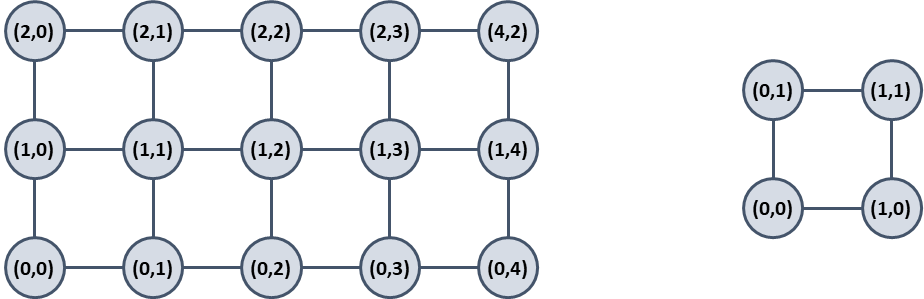
\includegraphics[width=12cm]{fig_01}
\caption{Grille (5,3) et grille (2,2)}
\end{figure}

Le graphe est implémenté par un dictionnaire d'adjacence où les clés sont les tuples, coordonnées d'un sommet. La valeur associée est une liste des sommets voisins. 


\begin{qexo}
Écrire la fonction \texttt{creer\_graphe(n:int, p:int) -> \{\}} permettant de créer le graphe d'une grille de \texttt{n} colonnes et \texttt{p} lignes.
\end{qexo}

\begin{exemple}
La grille $ 2 \times 2$ sera modélisée par le graphe suivant :

\begin{lstlisting}
>>> G2 =  creer_graphe(2,2)
>>> G2
        {(0, 0): [(1, 0), (0, 1)],
        (1, 0): [(1, 1), (0, 0)],
        (0, 1): [(1, 1), (0, 0)],
        (1, 1): [(0, 1), (1, 0)]}
\end{lstlisting}
\end{exemple}

On souhaite afficher ce graphe en utilisant \texttt{matplotlib}. Pour cela, on va commencer par tracer chacune des arêtes puis chacun des sommets. 

\begin{qexo}Écrire la fonction \texttt{get\_sommets(G:dict) -> (list,list)} renvoyant deux listes \texttt{les\_x} et \texttt{les\_y} contenant respectivement les abscisses des sommets et les ordonnées des sommets.
\end{qexo}


\begin{exemple}
Dans l'exemple qui suit, les coordonnées de sommets peuvent être dans un ordre différent. 
\begin{lstlisting}
>>> les_sx, les_sy = get_sommets(G2)
>>> les_sx, les_sy
        ([0, 1, 0, 1], [0, 0, 1, 1])
\end{lstlisting}
\end{exemple}


\begin{qexo}
Écrire la fonction \texttt{trace\_sommets(G:dict, couleur : str) -> None} qui trace sur la figure courante les sommets en utilisant un point coloré.

Exemples : pour tracer avec des points rouge on utilise la fonction suivante : \texttt{plt.plot(x,y,'r.')};  en bleu : \texttt{plt.plot(x,y,'b.')}, en noir : \texttt{plt.plot(x,y,'k.') }.
\end{qexo}

\begin{qexo}
Écrire la fonction \texttt{get\_aretes(G:dict) -> list} renvoyant la liste des arêtes du graphe sous la forme d'une liste de listes de tuples. Une arête est donc une liste de sommets où les sommets sont des tuples. Les arêtes ne devront être présentes qu'une fois.
\end{qexo}

\begin{exemple}
Dans l'exemple qui suit, l'ordre des arêtes peut être dans un ordre différent. Pour une arête donnée, les sommets peuvent aussi être dans un ordre différent.
\begin{lstlisting}
>>> get_aretes(G2)
	[[(0, 0), (1, 0)], [(0, 0), (0, 1)], [(1, 0), (1, 1)], [(0, 1), (1, 1)]]
\end{lstlisting}
\end{exemple}

\begin{qexo}
Écrire la fonction \texttt{trace\_arete(s1:tuple, s2:tuple, couleur : str , epaisseur : int ) -> None} qui trace une arête reliant les sommets \texttt{s1} et \texttt{s2} sur la figure courante. 

Exemple : pour tracer l'arête [(0,2),(1,2)] en bleu avec une épaisseur de 2, il faut utiliser l'instruction : \texttt{plt.plot([0,1],[2,2],'b',linewidth=2)}.
\end{qexo}


\begin{qexo}
Écrire la fonction \texttt{trace\_graphe(G:dict,couleur : str,epaisseur : int) -> None} qui permet de tracer les sommets et les arêtes du graphe \texttt{G} sur la figure courante. Tracer le graphe en rouge avec une épaissuer de 1 pour obtenir la figure ci-dessous.
\end{qexo}

\begin{figure}[!h]\centering
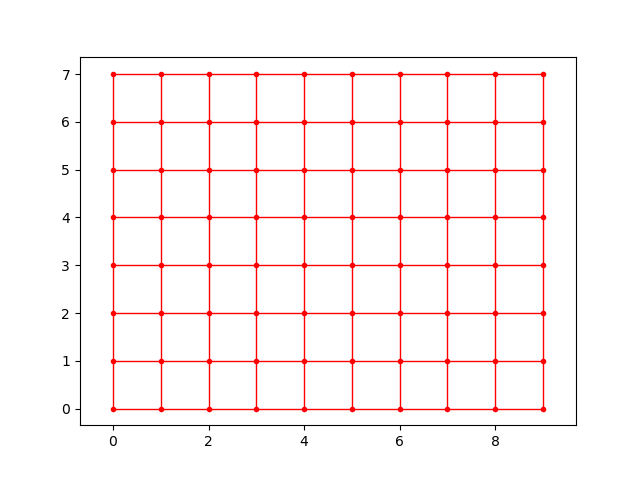
\includegraphics[width=6cm]{grille_10_8}
\vspace{-0.6cm}
\caption{Tracé d'un graphe grille de 10 colonnes et 8 lignes}
\end{figure}


\newpage
\subsection*{TP : Génération d'un labyrinthe}

\setcounter{cexo}{0}

L'objectif de ce TP est de générer un labyrinthe. Un labyrinthe est un graphe qui contient tous les sommets de la grille et un certain nombre d'arêtes pour les relier.
Pour obtenir un labyrinthe aléatoirement on réalise un parcours de la grille obtenue dans l'activité préparatoire.
Pour cela il faut visiter l'ensemble des sommets de la grille et conserver les chemins qui ont permis cette découverte. Sommets et arêtes seront stockés dans un graphe appelé labyrinthe.

\begin{figure}[!h]\centering
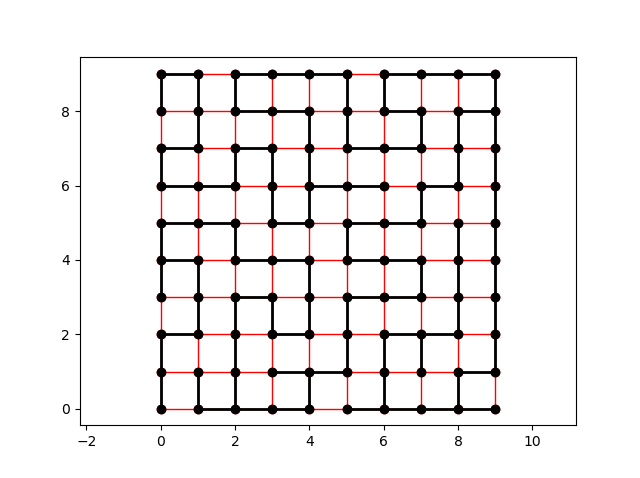
\includegraphics[width=0.4\textwidth]{exemple_laby.png}
\caption{Exemple de labyrinthe obtenu sur une grille 10*10}
\end{figure}


Viendra ensuite le moment de résoudre ce labyrinthe : ce sera l'objectif de la dernière partie. Il faudra alors être capable de trouver le chemin qui permet d'aller du coin inférieur gauche (départ) au coin supérieur droit (arrivée) en n'empruntant que les lignes (arêtes) du labyrinthe. 

	
\begin{figure}[!h]\centering
	\begin{minipage}{.4\textwidth}
	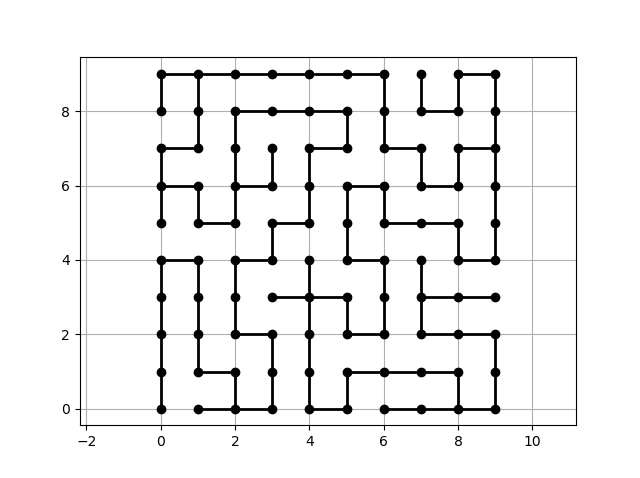
\includegraphics[width=\textwidth]{labyrinthe.png}
	\end{minipage}
\hspace{0.5 cm}	
	\begin{minipage}{.4\textwidth}
	
		\includegraphics[width=\textwidth]{labyrinthe résolu.png}
		
	\end{minipage}
\caption{Un labyrinthe et ce même labyrinthe résolu}
\end{figure}


\newpage

\section{Ajouter une arête dans un graphe}
Pour générer un labyrinthe il faut construire un graphe vide puis ajouter une arête à chaque fois que l'on découvre un sommet.



\begin{qexo}
Écrire la fonction \texttt{ajouter\_arete(G:dict, s1:tuple, s2:tuple) -> None} qui permet d'ajouter l'arête \texttt{([s1,s2])} au graphe \texttt{G}. 
\end{qexo}

\begin{exemple}
On reprend le graphe noté \texttt{G2} précédemment. 
\begin{lstlisting}
>>> ajouter_arete(G2,(1,0),(2,0))
>>> G2
        {(0, 0): [(1, 0), (0, 1)],
        (1, 0): [(1, 1), (0, 0), (2, 0)],
        (0, 1): [(1, 1), (0, 0)],
        (1, 1): [(0, 1), (1, 0)],
        (2, 0): [(1, 0)]}
\end{lstlisting}
\end{exemple}


\textbf{Bien penser aux éléments suivants :} ajouter une arête entre les sommets \texttt{s1} et \texttt{s2} consiste :
\begin{itemize}
\item à ajouter le sommet \texttt{s1} dans le graphe si ce sommet n'existait pas : dans ce cas il faut commencer une nouvelle liste de ses voisins avec son premier voisin \texttt{s2};
\item à ajouter le sommet \texttt{s2} dans le graphe si ce sommet n'existait pas : dans ce cas il faut commencer une nouvelle liste de ses voisins avec son premier voisin \texttt{s1};
\item à ajouter \texttt{s1} (respectivement \texttt{s2}) dans la listes des voisins de \texttt{s2} (resp. \texttt{s1}) dans le cas où le sommet \texttt{s2} (resp. \texttt{s1}) existait déjà.
\end{itemize}


\section{Marquages des noeuds visités}
%La programmation des parcours peut s'avérer difficile la première fois. Pour mieux visualiser les choses on propose dans ce TP d'afficher au cours du parcours :
%\begin{itemize}
%\item la grille initiale (graphe initial) en rouge en trait fin;
%\item les sommets déjà découverts avec des points noirs ou gris ;
%\item la file des sommets à explorer avec des croix bleues, la tête de la file aparaissant en plus gros.
%\end{itemize}

%\subsection{Marquage des noeuds visités}
On propose de marquer les sommets en utilisant un dictionnaire noté \texttt{visited}:
\begin{itemize}
\item
 Initialement, tous les sommets sont blancs. On dira qu’un sommet blanc n’a pas encore été
découvert.
\item Lorsqu’un sommet est “découvert” (autrement dit, quand on arrive pour la première fois sur
ce sommet), il est colorié en gris. Le sommet reste gris tant qu’il reste des successeurs de ce
sommet qui sont blancs (autrement dit, qui n’ont pas encore été découverts).
\item Un sommet est colorié en noir lorsque tous ses successeurs sont gris ou noirs (autrement dit,
lorsqu’ils ont tous été découverts).

\end{itemize}


Ce dictionnaire contiendra tous les sommets de la grille.

On leur associera le caractère \textbf{'W'} pour blanc (\textbf{W}hite), \textbf{'G'} pour gris et \textbf{'K'} pour noir (blac\textbf{K}).

\begin{qexo}
Créer un graphe \texttt{G} associé à une grille initiale de 5*5. L'afficher (épaisseur 1, en rouge).%
\end{qexo}

\begin{qexo}
Créer un dictionnaire \texttt{visited} associé à cette grille ayant ses valeurs toutes à \texttt{'W'}.
\end{qexo}

\begin{qexo}
Créer une fonction \texttt{trace\_visites} qui prend pour argument un dictionnaire \texttt{v} des sommets découverts et trace les noeuds découverts en gris ou en noir.

 (\textit{Rappel : tracé avec  points noirs : \texttt{plt.plot(x,y,'ko')}     / avec des points gris : \texttt{plt.plot(x,y,'o',color='grey')} )}
\end{qexo}

\begin{qexo}
Test : Après avoir modifié arbitrairement le dictionnaire \texttt{visited} pour le test (ajouter arbitrairement des noeuds en gris et en noir), le tracer sur la même figure que la grille.
\end{qexo}


%\subsection{Affichage des noeuds de la file}

%On propose de tester l'affichage avec par exemple cette file : \texttt{$file=deque([(1,0),(2,1),(4,3)]$}.

%\begin{qexo}
%Ecrire une fonction \texttt{trace\_file} qui prend pour argument une file \texttt{f} et trace avec une croix bleue de taille 8 les noeuds de la file et avec une croix bleue de taille 16 la tête de file. Attention de ne pas modifier la file ! (\textit{Rappel : tracé avec croix bleues de taille 8 : \texttt{plt.plot(x,y,'gx',markersize=8))}  )}
%\end{qexo}

%\begin{qexo}
%Test : Tracer sur la même figure les noeuds de la file ci-dessus. Vérifier que la file n'est pas modifiée par le tracé.
%\end{qexo}

%\subsection{Affichage de l'état du graphe}
%\begin{qexo}
%En utilisant les fonctions précédentes écrire une fonction \texttt{trace\_etat} prenant pour argument un graphe \texttt{G}, un dictionnaire \texttt{v} des sommets découverts et une file \texttt{f} qui efface la figure précédente (\texttt {plt.clf()}) puis trace le graphe en rouge, les noeuds visités en gris/noir et la file en bleu. 
%\end{qexo}


\section{Génération d'un labyrinthe par parcours en largeur}


On propose de travailler par étape en modifiant successivement la fonction pour aboutir à l'agorithme complet du parcours en largeur.
La fonction aura pour argument systématiquement le graphe à parcourir \texttt{G} et un noeud de départ \texttt{depart}. Vous penserez à modifier la coloration des sommets (via le dictionnaire \texttt{visited} (= dictionnaire des sommets découverts) au fur et à mesure.

\subsection{Initialisation}
\begin{qexo}
Ecrire une fonction \texttt{parcours\_largeur\_init}, qui initialise le dictionnaire des sommets découverts (tout à 'W'), crée une file ne contenant que le noeud de départ et trace l'état obtenu en utilisant votre fonction \texttt{trace\_visites}.
\end{qexo}


\subsection{Première étape : visite des voisins}
\begin{qexo}
Modifier la fonction précédente pour obtenir la fonction \texttt{parcours\_largeur\_etape1}, qui explore le premier sommet (la tête de file). On entend ici par "explorer", découvrir ses voisins, les ajouter dans la file s'ils n'ont pas été déjà découverts. Tracer aussi l'état obtenu. 
\end{qexo}

\subsection{Algorithme complet}
\begin{qexo}
Modifier la fonction précédente pour obtenir la fonction \texttt{parcours\_largeur\_complet}, qui continuera à explorer les voisins tant que la file n'est pas vide. A chaque étape (à chaque tour de boucle) vous pouvez tracer l'état, tracer une arête pour indiquer le chemin parcouru, et ajouter l'instruction \texttt{plt.pause(0.5)} de façon à voir progressivement le parcours du graphe.
\end{qexo}

\textit{Vous pouvez utiliser la note en bas de page pour ajouter de l'aléatoire au parcours.}

\subsection{Algorithme complet avec création du labyrinthe}
Il est maintenant possible de créer le labyrinthe.

\begin{qexo}
Modifier la fonction précédente pour obtenir la fonction \texttt{labyrinthe\_largeur}, qui construit le graphe labyrinthe \texttt{L} au fur et à mesure du parcours. Cette fonction retourne le graphe labyrinthe. Vous pouvez tracer à chaque étape le labyrinthe en trait plus épais noir. 
\end{qexo}

\vspace{-0.8cm}
\begin{figure}[!h]\centering
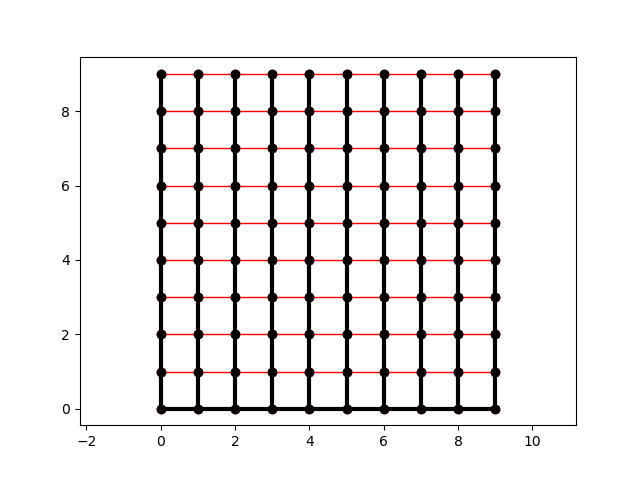
\includegraphics[width=0.4\textwidth]{laby_larg.png}
\vspace{-0.7cm}
\caption{Exemple de labyrinthe obtenu sur une grille 10*10 par parcours en largeur}

\end{figure}



\textbf{Note :} Comme vous pouvez le constater, le coté aléatoire de ce labyrinthe est discutable :). Il est possible de mélanger une liste en utilisant le module \texttt{random} : \texttt{random.shuffle(voisins)} ce qui permet de mélanger la liste de tuples voisins.


\section{Génération d'un labyrinthe par parcours en profondeur}
\begin{qexo}
Modifier l'algorithme \texttt{parcours\_profondeur}  pour réaliser le marquage des sommets comme proposé (gris = sommet "découvert", noir = sommet dont tous les voisins ont été découverts).
\end{qexo}

\begin{qexo}
Etablir la fonction \texttt{labyrinthe\_profondeur}, qui construit le graphe labyrinthe \texttt{L} par un parcours en profondeur. Vous pouvez tracer à chaque étape le labyrinthe en trait plus épais noir. 
\end{qexo}

\section{Résolution du labyrinthe}

Il est possible de résoudre le labyrinthe en utilisant un parcours en largeur ou un parcours en profondeur.

\begin{qexo} Écrire la fonction \texttt{resolution\_largeur(G:dict, s:tuple) -> list} qui permet de résoudre le labyrinthe en utilisant un parcours en largeur. Cette fonction renvoie la liste des sommets permettant d’atteindre le sommet en haut à droite depuis le sommet en bas à gauche.
\end{qexo}

\begin{qexo}
Afficher en trait épais bleu la solution donnée par le parcours en largeur.
\end{qexo}

\begin{qexo}
Répondre aux mêmes questions en utilisant un parcours en profondeur.
\end{qexo}



\end{document}